\section{Introduction}
\label{sec:intro}

Mechanistic interpretability can currently do supervised steering well
or unsupervised steering poorly. The Google DeepMind mechanistic
interpretability team has pivoted from ambitious reverse-engineering to
pragmatic interpretability judged on proxy tasks, and has deprioritized
SAE research: SAE probes did not generalize better out of distribution,
and SAEs did not beat a steering vector built from one contrastive pair
of prompts at suppressing a model's awareness of being
evaluated~\cite{gdmprogress2025}. On current benchmarks the supervised
difference of means steers better than SAE latents, though worse than
prompting~\cite{wu2025axbenchsteeringllmssimple}. But a supervised
method finds only the concepts an experimenter already has labels for,
and a direction that changes outputs as intended need not be one the
model computes with: a subspace intervention optimized for its effect
can instead activate a dormant pathway~\cite{makelov2023}.

The dominant unsupervised paradigm is the sparse autoencoder (SAE), which
approximates a model's hidden state by a few discrete features drawn
from an overcomplete dictionary, first with a $\relu$ activation and a
sparsity loss~\cite{cunningham2023,bricken2023} and more recently with a
$\topk$ activation and no sparsity loss~\cite{gao2024}. The motivation is
to decompile a model to a finite state machine, and such a machine is
only as interpretable as an enumeration of its states: even a mixture of
two structureless processes, one constant and one a fair coin, needs
infinitely many states to track which component is generating, so the
structure lives in how the components overlap~\cite{crutchfield2026}.
Ideally interpretability would give guarantees about the computational
process a model uses, with features that are causal, disentangled and
closed-form. SAE features can fail all three, and are expensive besides.

\subsection{Problems with SAE features}

\paragraph{Features are not disentangled.}
A representation is disentangled when a change in one factor of variation
changes one factor of the representation~\cite{locatello2019}. A
persistent problem with SAEs is feature absorption~\cite{chanin2025}:
when one feature implies another, sparsity is better served by folding
the general feature's direction into the specific feature's latent and
switching the general latent off there, so a latent that looks
monosemantic silently fails to fire on some inputs that have its feature
(a ``starts with S'' latent that is silent on ``short''). A related
failure, feature composition~\cite{bussmann2025}, merges concepts that
co-occur into one latent, so neither can be set without the other. Nested
and hierarchical SAEs reduce both (Section~\ref{sec:background}).

\paragraph{Features are not cleanly causal.}
Sparsity trades off against reconstruction fidelity~\cite{gao2024}, and
steering with an SAE feature is rarely clean: adding its decoder
direction moves the logits differently in different contexts and
disturbs unrelated downstream features. How much varies by feature and is
partly predictable before intervening, from the crowding of its decoder
direction and its direct effect on the logits, though which predictor
works differs between models and dictionaries~\cite{duan2026}.

\paragraph{Features are not closed-form.}
A major concern is how well an interpretability technique generalizes out
of distribution, and ideally behavior could be inferred from the model's
weights alone. Bilinear MLPs make this partly possible: the interaction
matrix of any output direction can be eigendecomposed without data,
although in deep models the output directions to decompose still come
from data-dependent SAEs~\cite{pearce2025}.

\paragraph{Forward passes are expensive.}
Although only a handful of features are active for a given input, the
entire feature space is computed for each
sample~\cite{gao2024,mudide2025}. Mixture-of-experts (MoE) SAE variants
cut that cost by dividing the feature space between smaller submodules
(Section~\ref{sec:background}).

\subsection{Contrastive classifiers}

Less explored is the effect of the structure an MoE architecture imposes
on the interpretability of feature space. A common approach to interpreting
features at scale is to have an LLM explain each feature from its
activating examples and score the explanation by how well an LLM judge,
given only the explanation, separates activating from non-activating
contexts~\cite{paulo2025}. With an unstructured feature space it quickly
becomes intractable to interpret every combination of features this way,
but the same technique applies to expert routings. The ReLU feed-forward
layers of a trained transformer can themselves be split into experts of
co-activating neurons, keeping over 95\% of performance with 10--30\% of
the parameters~\cite{zhang2022}. Language models appear to represent a
categorical concept as a simplex whose vertices are the vectors of its
values, with hierarchically related concepts in orthogonal subspaces, so
that a hierarchy is a direct sum of simplices; differences between value
vectors are the steering vectors of binary contrasts~\cite{park2025}.

We conjecture that MoEfying a representation into classifiers can reveal
such latent contrastive steering vectors, since swapping a classifier's
choice writes exactly such a difference. Existing MoE SAEs route similar
inputs to the same expert~\cite{mudide2025} and score an expert as
specialized when its features resemble each other and not other
experts'~\cite{xu2025redundancydiversespecializedmultiexpert}.
Contrastive learning wants the opposite: inputs at opposite ends of a
shared axis. The Ontologizer\footnote{Gene Ontology terms were a source of
inspiration for the name, which this work shares with Ontologizer, a tool
for Gene Ontology term enrichment analysis~\cite{bauer2008}; the two are
separate projects.} decomposes a representation space into a set of such
contrastive classifiers. Each \emph{head} is a $k$-way classifier over
its input, and each of its \emph{entries} writes a representative vector,
its \emph{atom}. An input is encoded as one \emph{assignment} per head and
reconstructed from the atoms its assignments select, by a stack of layers
each of which reads what the layers before it left unexplained.
Interpretability value is then expected from \emph{MoEfication}, in an
extended sense of the term~\cite{zhang2022}: a decomposition of the space
into small classification tasks, one per head, each nameable in
isolation, whose within-head entry swaps are steering moves.
Figure~\ref{fig:teaser} shows the soft code's steering primitive, measured.

\begin{figure}[tp]\centering
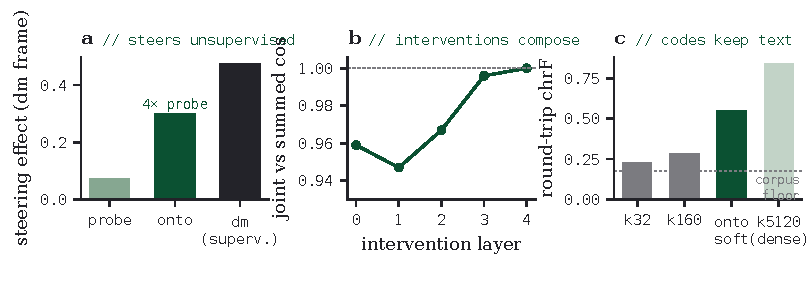
\includegraphics[width=\linewidth]{figures/fig-teaser.pdf}
\caption[The steering primitive, measured]{The softmax Ontologizer's
steering primitive, measured. (a) Forcing an entry moves decodes along
the supervised difference-of-means direction $0.64\times$ as far as
supervised steering itself and $4\times$ as far as probe directions
(\texttt{resid\_nc\_hm}; Table~\ref{tab:steer-overlay}). (b) Joint
two-head interventions point where the summed single interventions point,
exactly in the final layer (\texttt{resid\_nc}; Section~\ref{sec:formal}).
(c) The sparse SAEs' codes lose most text before any intervention
(round-trip chrF 0.23--0.28 against a 0.18 corpus floor) while the soft
code keeps it (0.55); the dense \texttt{k5120} keeps more but is not a
sparse code (Appendix~\ref{sec:textfid}).}
\label{fig:teaser}
\end{figure}

\subsection{Disjoint support}
\label{sec:intro-disjoint}

Concatenated heads (\texttt{ConcatDictBlock}) give each head its own block
of the dictionary's coordinates, so the atoms of different heads have
disjoint supports by construction. Disjoint support is the strong form of
orthogonality: for non-negative atoms the two coincide
(Eq.~\eqref{eq:disjoint}), while signed vectors can be orthogonal by
cancellation and share every coordinate. Summed heads can only be asked
for it, and they do not deliver it: no trained summed model partitions its
coordinates between heads, and penalizing the overlap on GPT-2 produced a
partition only by moving atom energy into directions the decoder discards
or shrinks, where reconstruction cannot see it (Section~\ref{sec:disjoint},
Appendix~\ref{sec:support}). Disjoint support bears on each of the four
problems above, though unequally. In each case the guarantee holds between
the heads of one layer and in the dictionary; what reaches the output
passes through a shared decoder, which in general maps the heads' blocks
onto overlapping subspaces.

\paragraph{Disentanglement.}
Absorption needs two things: a general latent that switches off where a
specific one fires, and a specific latent whose direction takes over the
general one's. The head structure removes the first, since every head
writes on every input, choosing among its entries, and so cannot fall
silent where its feature applies. Disjoint support removes the second: no entry of one
head can carry a component of another head's block. Feature composition
is discouraged rather than excluded. Heads already make the code factorial,
$k^h$ codes from $hk$ atoms, so concepts that vary independently can take
separate heads, and theory says when an efficient code would put them
there. Under a quadratic cost on activity and a bound on the
weights~\cite{whittington2023,dorrell2025}, a non-negative code gives two
variables disjoint supports when their joint range is spread enough,
roughly when every combination of their extreme values
occurs~\cite{dorrell2025}. On SONAR the data meet that condition: of the
entry pairs of two heads that independence predicts at least ten times,
at most 0.24\% never occur in any layer of a SONAR model. The summed
models carry no such cost and do not partition
(Appendix~\ref{sec:support}); concatenation imposes the partition by
construction. Nothing yet forces a head to hold one concept rather than a
conjunction of two. Nor can any method that sees only the data recover its
factors without inductive biases, on the model and on the data, that
match~\cite{locatello2019}. The heads are such a bias, and
Section~\ref{sec:seeds} measures how far it reaches.

\paragraph{Causality.}
An SAE's steering is unclean partly because its decoder directions crowd
one another~\cite{duan2026}. Between heads, nothing crowds in the
dictionary. Forcing a head's entry rewrites only that head's block of the
layer's output, orthogonal to everything the other heads of the layer
write, so interventions on different heads move the output along
orthogonal directions and each head's contribution can be read off its
own block. Summed heads also compose additively, by linearity, but their
writes overlap, so one head's contribution cannot be read apart from the
others'. What disjoint support does not govern is how the other heads
read a stepped input. Measured on the summed models by re-encoding, an
input-space step moves as many other heads as a random step of its
length, because the heads sit almost on their decision boundaries and
downstream layers reclassify a changed residual
(Section~\ref{sec:entangle}). A disjoint write removes neither cause.

\paragraph{Closed form.}
A static reading of the dictionary, which interprets a head from its
atoms without data, needs heads that own disjoint coordinates as a
property of the weights, for every input rather than on the data measured
(Section~\ref{sec:disjoint}). In the summed models that premise fails:
each head's usage covers 52--98\% of the coordinates. Concatenated heads
supply it, and when each head's decoder block has full column rank, every
part of a head's atoms reaches the output, unlike the partitions the
overlap penalty produced (Appendices~\ref{sec:support}
and~\ref{sec:concatgeom}). It is a premise, not yet a reading:
decoding atoms through the paired decoder has not described what an entry
does in the models scored so far, none of them with concatenated heads
(Section~\ref{sec:autointerp}).

\paragraph{Cost.}
Disjoint support does least here. Concatenation divides the dictionary
among the heads, so at matched width $e$ each head stores $k$ atoms of
$e/h$ coordinates rather than $e$, $h$ times fewer dictionary parameters,
and a hard code's dictionary step is $h$ lookups that together write one
$e$-vector. But the classifier still scores all $hk$ entries for every
input, as an SAE scores all of its latents, so the forward pass is no
cheaper on the encoder side. Narrow blocks also cost reconstruction. At
$d_{\mathrm{head}}{=}k$, where each head's block is just wide enough for
its atoms, concatenated heads had the worst held-out error of the GPT-2
orthant arms ($\fvu$ $0.416$ against $0.154$--$0.293$;
Table~\ref{tab:orthant}); orthogonal atoms within a head need one
coordinate each there (Appendix~\ref{sec:concatgeom}).

\subsection{This document}

This document is the working record of that program. It compares a
softmax (soft-code) Ontologizer and a straight-through (hard-code) arm
against $\topk$ SAEs on SONAR sentence embeddings under the same whitened
objective, and the hard code on GPT-2 small residuals.
Section~\ref{sec:background} places the architecture among its nearest
neighbors and Section~\ref{sec:frame} states what the evaluation asks;
the architecture follows in Section~\ref{sec:methods} and the results in
Sections~\ref{sec:results}--\ref{sec:geom}.

\section{Background}
\label{sec:background}

No single line of prior work covers this combination; each commitment has
a nearest neighbor.

\paragraph{Quantizers and discrete latents.}
A \texttt{DictBlock} layer --- $h$ heads, each a softmax over $k$ entries,
their atoms summed --- is a soft additive quantizer~\cite{babenko2014}, the
generalization of product quantization~\cite{jegou2011} in which every
codebook spans the whole space rather than its own block of coordinates
(\texttt{ConcatDictBlock} is a product quantizer in the dictionary space).
Composite quantization~\cite{zhang2014composite} lies between the two: it
holds the summed inner products between different codebooks' codewords at
a constant, which product quantization's disjoint blocks fix at zero, and
optimized product quantization~\cite{ge2014} learns the rotation that sets
the blocks.
In dictionary-learning terms a hard head is vector quantization, one atom
at unit coefficient, and a sum of heads lies between vector quantization
and free sparse coding, with exactly one unit-coefficient atom per
codebook; under the gain--shape split (Eq.~\eqref{eq:y_norm}) each layer
is gain--shape VQ, its one coefficient the residual's measured norm rather
than a quantized index~\cite{aharon2006}.
The residual layer stack is a softmax relaxation of residual (multi-stage)
VQ, the quantizer of neural codecs such as SoundStream~\cite{zeghidour2021},
which picks each stage's code by nearest neighbor and judges codes only by
rate and perceived quality, never by what a codeword means; residual VQ has
also been applied to SONAR space itself, with 64 codebooks of 8192
entries~\cite{lcmteam2024largeconceptmodelslanguage}. The straight-through
arm (Section~\ref{sec:ste}) makes the analogy literal: with an argmax
forward and the softmax's gradient in the backward pass --- the
straight-through estimator~\cite{bengio2013} in its categorical
form~\cite{jang2017} --- it is a residual additive quantizer with
non-negative atoms, whose codewords are picked by learned classifiers
rather than by nearest-codeword search. Vectors of categorical variables
trained with straight-through gradients are also the latent state of
discrete world models~\cite{hafner2021,hafner2023}, which sample each
categorical from the softmax the backward differentiates rather than take
its argmax (DreamerV3 also mixes 1\% uniform into it~\cite{hafner2023});
there the codes are compressed state, never read as features. Codebook Features~\cite{tamkin2023} is the
closest interpretability ancestor: it finetunes VQ bottlenecks into
a network, one codebook per attention head ahead of the shared output
projection (in effect \texttt{ConcatDictBlock} with its shared decoder),
and steers by substituting codes, including swapping one state's code for
another's in a synthetic finite-state task. But its codes are chosen by
cosine similarity to the codes themselves rather than by a classifier,
read one at a time as present-or-absent features, and scored on their
target alone, with no defined set of operations and no measure of what
else an intervention changes.

\paragraph{Routed and mixture-of-experts dictionaries.}
Switch SAEs~\cite{mudide2025} route each activation to one of several
expert $\topk$ SAEs to cut training compute;
routing gathers similar inputs, and experts duplicate some features
(5--10\% of decoder directions have a near-copy in another expert), which
Xu et al.\ describe as experts collapsing into redundant ensembles and
counter by activating several experts per
input~\cite{xu2025redundancydiversespecializedmultiexpert}. A head layer is
the dual arrangement --- every head fires, choosing one entry --- and the
hard stack's heads partition near-independently
(Figure~\ref{fig:headnmi}), while in the reference softmax model a head's
decode directions repel (Section~\ref{sec:prelim-orth}): a head there is a
contrast set rather than the coherent cluster that MoE work counts as a
specialized expert. MoEfication~\cite{zhang2022} supplies the frame's name,
but its experts are found post hoc in already-trained layers and several
are active per input; a head's entries instead exclude one another, and
the partition is the training objective's own discovery.

\paragraph{Deep clustering.}
Each head is a $k$-way classifier trained without labels, the setting of
deep clustering, which supplies two of the objective's terms. The
batch-mean entropy term $\mathrm{KL}_m$ (Eq.~\eqref{eq:KL}) is the
anti-collapse term of contrastive clustering~\cite{li2021cc} and
SCAN~\cite{vangansbeke2020scan}, which keeps a clusterer from assigning
most inputs to a few clusters, and the partition-consensus statistic
$\mathrm{KL}_{\mathrm{pwak}}$ (Eq.~\eqref{eq:stats}) pulls each
assignment toward a stop-gradient average of its neighbors', in the line
of DEC's self-training target~\cite{xie2016dec} and SCAN's neighbor
agreement. Those methods learn one clustering of a learned embedding and
are judged by agreement with class labels; here many heads partition a
fixed embedding at once, trained only through reconstruction, and the
partitions are the code.

\paragraph{Structured SAEs.}
Sparse autoencoders recover features in superposition~\cite{elhage2022}
as sparse combinations of directions from an overcomplete
dictionary~\cite{cunningham2023,bricken2023}; the $\topk$ baselines here
are k-sparse autoencoders~\cite{makhzani2014} trained as in Gao et
al.~\cite{gao2024}. The field's main structure axis is nesting by scale:
Matryoshka SAEs~\cite{bussmann2025} carry the nested loss of Matryoshka
representation learning~\cite{kusupati2022} into a dictionary to curb
feature absorption~\cite{chanin2025}, and Tree SAEs~\cite{cao2026} learn
explicit parent--child pairs by gating each child latent on an assigned
parent. Grouping is a second axis: subspace-aware SAEs~\cite{dalili2026}
tie latents into rank-$r$ blocks and sparsify across blocks, so that a
group is a subspace with free signed coordinates, and
OrtSAEs~\cite{korznikov2025} penalize each decoder direction's cosine with
its nearest neighbor. Rung 3 (\texttt{k32\_p5}) imports the Matryoshka
nested-prefix loss into the ladder, with five equal blocks rather than the
doubling block sizes of~\cite{bussmann2025}, a log spacing that Matryoshka
representation learning found better than uniform~\cite{kusupati2022}.
The Ontologizer's axis is instead \emph{partition into exhaustive,
mutually exclusive heads}, and the geometry such heads ask for has a
theory: in Elhage et al.'s toy models, a set of features of which only one
is active at a time shares a subspace with negative interference inside
it, while separate sets take mutually orthogonal
subspaces~\cite{elhage2022}. A head imposes the first arrangement by
construction and asks for the second (Section~\ref{sec:disjoint}).
Outside dictionary learning, Huang and Hahn~\cite{huang2025decomposing}
partition a residual stream without supervision into mutually independent
orthogonal subspaces, on the hypothesis that each holds a group of
mutually exclusive features; their subspaces carry continuous activations
where a head names one of $k$ values. Post hoc, co-occurring latents of
LLM SAEs cluster in decoder space by document genre~\cite{li2024geometry},
the co-firing structure \texttt{headstruct.py} finds among SONAR SAE
latents in place of categorical groups (Appendix~\ref{sec:categorical}).
Each of these asks whether an architectural commitment buys
interpretability that code density alone does not explain. The autointerp
results below answer ``not per-latent describability''; the
description-coherence view is where the partition begins to pay,
suggestively and on the one Ontologizer it scores.

\paragraph{Embedding-space substrate.}
SAEs over dense text embeddings have become an active line of work:
interpreting and discretizing dense-retrieval
embeddings~\cite{park2025decodingdenseembeddingssparse} and aligning
sentence-embedding features with human concepts to steer
retrieval~\cite{shin2026aligningsentenceembeddingshuman}, while a
data-analysis toolkit builds interpretable document embeddings from a
token-level LLM SAE instead~\cite{jiang2026interpretableembeddingssparseautoencoders}.
All three rely on single-layer SAEs, $\topk$ or its BatchTopK variant, the
embedding SAEs on English retrieval encoders. None addresses SONAR, where
the stakes are higher --- Large Concept Models generate directly in SONAR
space~\cite{lcmteam2024largeconceptmodelslanguage} --- and where the paired
M2M100 decoder reads reconstructions and interventions back as text
without a trained inverter. Inverting a pooled sentence embedding
otherwise needs one, which recovers exact text only by iteratively
re-embedding and correcting its own
decodes~\cite{morris2023textembeddingsrevealalmost}; exact training-free
inversion is known only from a causal language model's per-token
states~\cite{nikolaou2025}, which a bidirectional, mean-pooled encoder
such as SONAR's does not provide. \texttt{textfid.py} and
\texttt{steerfid.py} decode in a single greedy pass through a decoder that
paraphrases and is fragile to small
perturbations~\cite{sonar,lcmteam2024largeconceptmodelslanguage}, so their
text-space numbers are lower bounds (Appendix~\ref{sec:steertext}).

\paragraph{Evaluation stance.}
SAEBench~\cite{karvonen2025} motivates judging a dictionary with many
instruments rather than by reconstruction at fixed sparsity; of its eight
metrics the battery adapts three to SONAR (a loss-recovered analogue
through the paired decoder, \texttt{textfid.py}; LLM-judged detection,
\texttt{autointerp.py}; $k_{\mathrm{probe}}$-sparse probing on 86
language labels, \texttt{langprobe.py}) and omits absorption, RAVEL,
unlearning, SCR and TPP. Description scoring uses the detection task of
the scaled autointerp pipeline~\cite{paulo2025}; unlike that pipeline we
score positives ranked just below the describing examples and report F1
rather than balanced accuracy, so our numbers are not on its scale.
Capacity is compared in bits rather than $\mathrm{L0}$, as
MDL-SAEs~\cite{ayonrinde2024} argue it should be, since an $\mathrm{L0}$
axis rewards ever wider dictionaries with ever fewer active latents; their
description length, summed per-latent usage entropy, is the realized-bits
estimator applied here to heads (Eq.~\eqref{eq:realized}).
AxBench~\cite{wu2025axbenchsteeringllmssimple} found that, averaged over
four Gemma-2 sites, prompting and then finetuning steer better than every
representation-based method. Among single directions only the difference
of means beats SAE latents, while a linear probe that ties the best
detectors steers worse than they do, and SAE latents chosen by their
autointerp labels also trail at concept detection. Detection and steering
dissociate, which supports judging a dictionary by what its directions do
--- the niche of \texttt{steerfid.py}'s
effect-against-collateral design at matched magnitude, which follows
Cunningham et al.'s scoring of feature edits against edit
magnitude~\cite{cunningham2023}, where AxBench instead tunes each method's
strength on held-out prompts. Song et
al.~\cite{song2025positionmechanisticinterpretabilityprioritize} argue
that run-to-run feature consistency should be an essential SAE evaluation
criterion, measured as the mean absolute cosine between decoder directions
matched one-to-one across seeds; \texttt{partition.py}'s Hungarian-matched
head NMI is its partition-level analogue for classifier heads, and
\texttt{splitting.py}'s match fractions a thresholded, activation-based
one. Wang et al.~\cite{wang2024} measure the same property as each latent's
maximum activation correlation with any latent of another run, against
model-seed and SAE-seed skylines. Korznikov et al.~\cite{korznikov2026}
retrain SAEs with the decoder frozen at a random initialization, or held
near it, or with the encoder frozen at random, and find them within a few
points of trained SAEs on autointerp, single-latent sparse probing and
RAVEL; the nulls here permute a trained model's own entries, latents or
rows, and do not measure what training adds over random components.
Decoding parameter directions through the paired decoder, to see whether
features can name themselves from weights alone, is a closed-form
instance of dataset-free feature synthesis, whose evaluation against
implanted ground truth finds that even the best such tools help humans
identify a planted trigger less than half the time~\cite{casper2023};
here the weights fail too. Two pieces have, to our knowledge, no close
analog: reading per-head routing as contrastive classification with a
causal intervention interface, and per-group coherence tests against
size-matched draws from the same dictionary, applied to trained heads and
to judge-written description texts as well as to geometry. Li et
al.~\cite{li2024geometry} test whole co-occurrence clusterings of SAE
latents against permuted labels.

\section{Evaluation frame}
\label{sec:frame}

The comparisons below were largely built on SAE-native terms ---
per-feature monosemanticity, sparse probing, reconstruction at matched
sparsity --- and we report them unchanged. But the Ontologizer's goal is
not a monosemantic dictionary. It is an \emph{unsupervised generator of
steering vectors}: each head is trained only by reconstruction pressure,
the hope is that a series of such classifiers finds the most natural
contrastive clusters in the embedding space, and within-head entry swaps
are the steering primitive (forcing head $i$ from its argmax entry to
entry $j'$ moves the decode along exactly the dimension head $i$
classifies).

Under this frame the evaluation questions are: (a)~what does contrast-set
structure cost in reconstruction (the Pareto and ladder); (b)~do trained
heads actually behave as contrastive classifiers (categorical form,
semantic anti-coherence); (c)~are the learned tasks \emph{natural} ---
nameable, stable across runs, aligned with generative factors of the data
(seed reproducibility, language and topic alignment); and (d)~is the
steering primitive good --- consistent effect, low collateral, at least
matching supervised diff-of-means vectors and SAE decoder-direction addition
(steering fidelity). Metrics that ask whether \emph{individual latents}
are concept-aligned remain informative about the SAE side but are the
wrong lens for classifier codes, and we flag them as such where they
appear. Figure~\ref{fig:teaser} shows the softmax Ontologizer on three
of question (d)'s criteria; the hard code steers less reliably than the
soft one (Section~\ref{sec:steer}).

Question (c) has a prerequisite that the original battery took for
granted: a head can only be named if it is the same head on every run.
Section~\ref{sec:seeds} tests that directly and finds it holds only
partly, and only in the first layer, which conditions every per-head
result in this document.
